\hypertarget{sendRCUcommand_8c}{
\section{send\-RCUcommand.c File Reference}
\label{sendRCUcommand_8c}\index{sendRCUcommand.c@{sendRCUcommand.c}}
}
The \hyperlink{group__rcu__sh}{rcu-sh}. 

{\tt \#include $<$stdio.h$>$}\par
{\tt \#include $<$string.h$>$}\par
{\tt \#include \char`\"{}memoryguard.h\char`\"{}}\par
{\tt \#include $<$linux/errno.h$>$}\par
{\tt \#include $<$signal.h$>$}\par
{\tt \#include \char`\"{}cmd\-Interpreter.h\char`\"{}}\par
{\tt \#include \char`\"{}dcsc\-Msg\-Buffer\-Interface.h\char`\"{}}\par
{\tt \#include \char`\"{}selectmap\-Interface.h\char`\"{}}\par
{\tt \#include \char`\"{}mrtimers.h\char`\"{}}\par
{\tt \#include \char`\"{}mrshellprim.h\char`\"{}}\par


Include dependency graph for send\-RCUcommand.c:\begin{figure}[H]
\begin{center}
\leavevmode
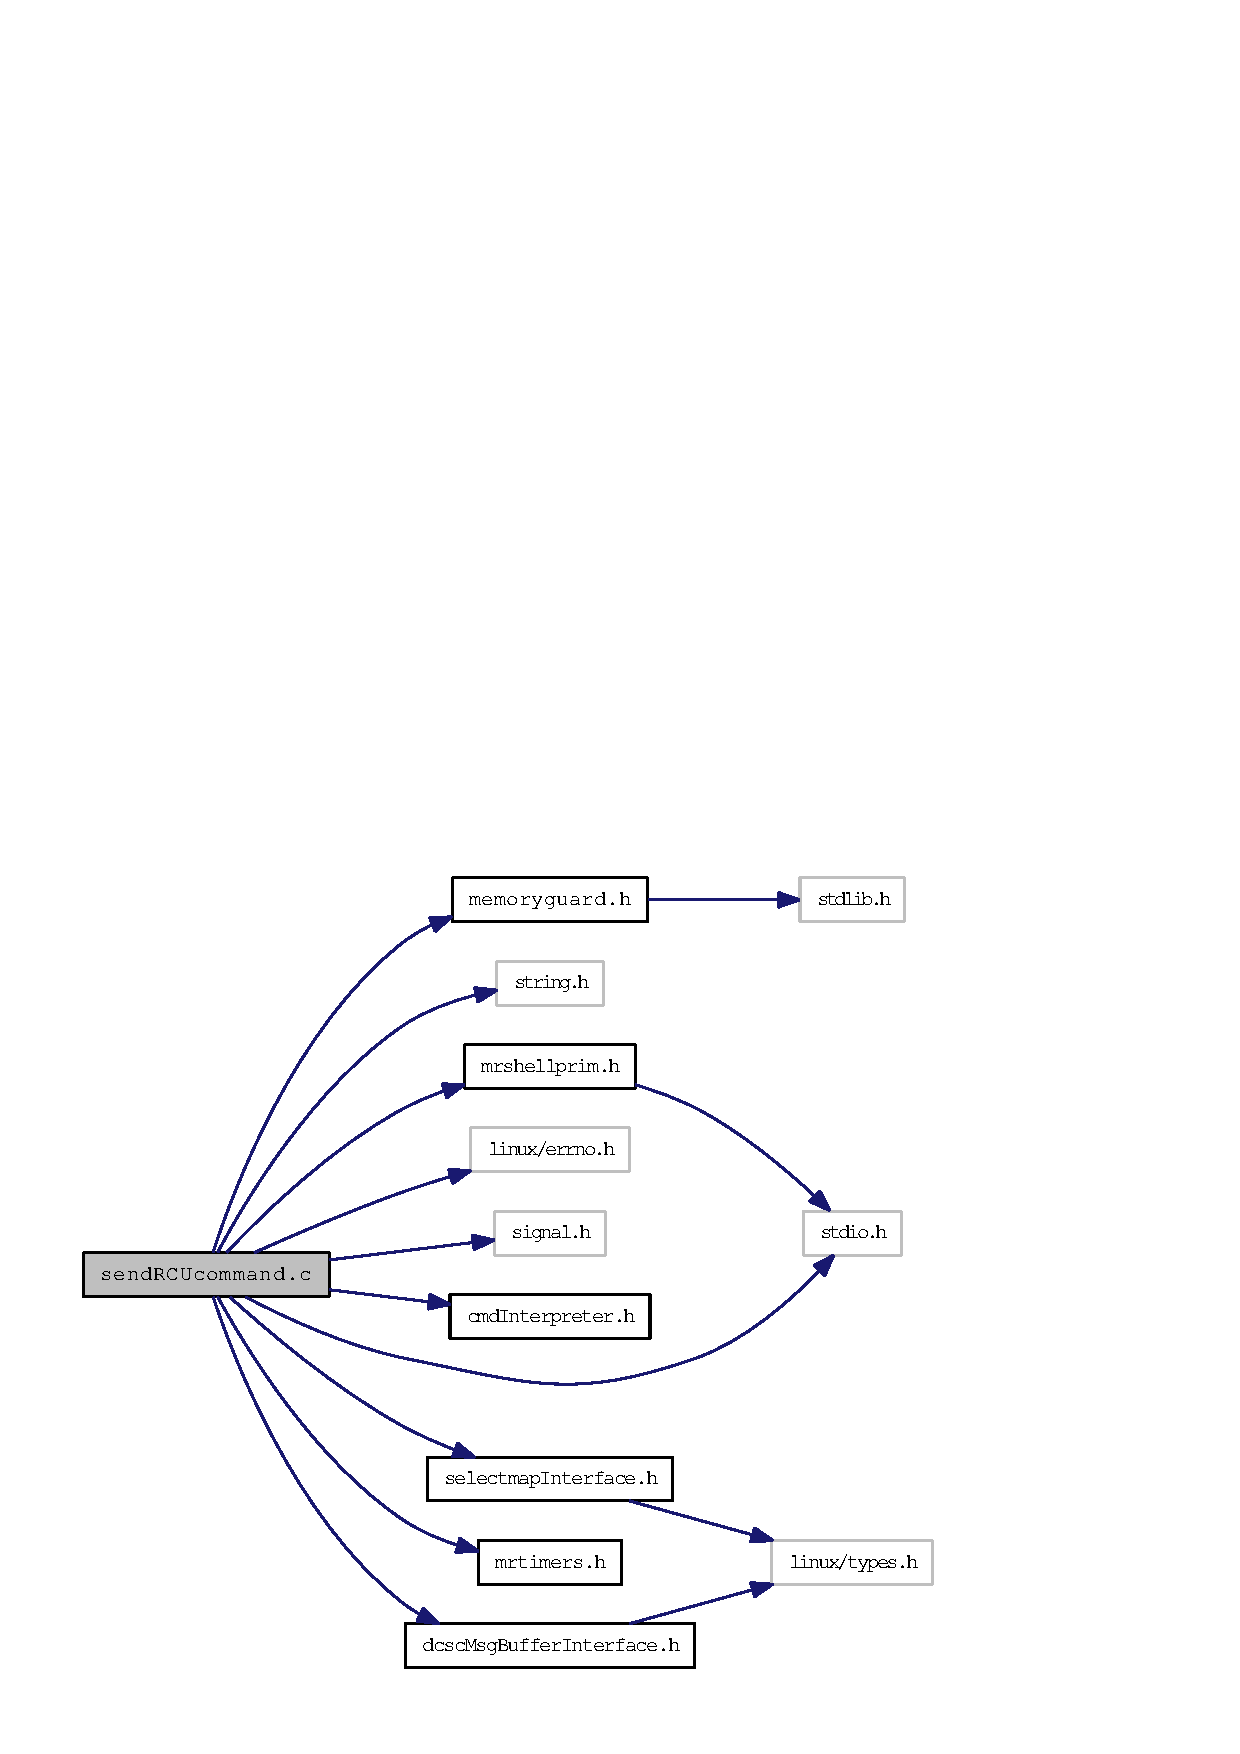
\includegraphics[width=226pt]{sendRCUcommand_8c__incl}
\end{center}
\end{figure}
\subsection*{Defines}
\begin{CompactItemize}
\item 
\#define \hyperlink{sendRCUcommand_8c_ff659880ee30289b3cfb7c93bc73e726}{ENABLE\_\-GETLINE}
\item 
\#define \hyperlink{sendRCUcommand_8c_7d71767838ad691171592b8bf69624ad}{promt}~\char`\"{}enter operation (h/i/q/r/w):\char`\"{}
\end{CompactItemize}
\subsection*{Functions}
\begin{CompactItemize}
\item 
char $\ast$ \hyperlink{sendRCUcommand_8c_a1a15405a6ce7f75a1d559feb39ce866}{Getline} (const char $\ast$prompt)
\item 
void \hyperlink{sendRCUcommand_8c_5bc9732aae5850cd5a7b8c7886f3384f}{Gl\_\-histadd} (char $\ast$buf)
\item 
void \hyperlink{sendRCUcommand_8c_47cf995bed43c4e6bc563073f5b8f607}{sigquit\-Handler} (int param)
\item 
int \hyperlink{sendRCUcommand_8c_22ebaf74d5c7bacab58b44ae963c85d6}{main} (int argc, char $\ast$$\ast$arg)
\end{CompactItemize}
\subsection*{Variables}
\begin{CompactItemize}
\item 
unsigned int \hyperlink{sendRCUcommand_8c_34fcfc606a53070425a87fce190ee38d}{g\_\-mr\-Shell\-Prim\-Dbg}
\item 
\hyperlink{structFctMode__t}{TFct\-Mode} \hyperlink{sendRCUcommand_8c_8481f9823ab837a716b4294324fd3def}{scan\-Mode\-No\-Error} = \{SCANMODE\_\-SILENT$|$SCANMODE\_\-FORCE\_\-TERMINATION, NULL, NULL\}
\item 
\hyperlink{structFctMode__t}{TFct\-Mode} \hyperlink{sendRCUcommand_8c_bae7cc25bf2667a9438fbb8ca696ae75}{scan\-Mode\-Main\-Options} = \{SCANMODE\_\-FORCE\_\-TERMINATION$|$SCANMODE\_\-READ\_\-ONE\_\-CMD$|$SCANMODE\_\-PERSISTENT, NULL, NULL\}
\item 
\hyperlink{structFctMode__t}{TFct\-Mode} \hyperlink{sendRCUcommand_8c_260fedd682f84c2bf63d9fbcf7a85a84}{scan\-Mode\-Shell\-Args} = \{SCANMODE\_\-FORCE\_\-TERMINATION, \char`\"{} \char`\"{}, NULL\}
\item 
\hyperlink{structArgDef__t}{TArg\-Def} \hyperlink{sendRCUcommand_8c_c5dd9bf9adc293400bcf4c9746e1624d}{shell\-Args} \mbox{[}$\,$\mbox{]}
\item 
\hyperlink{structArgDef__t}{TArg\-Def} \hyperlink{sendRCUcommand_8c_3f74ad6fcd7825c54ac293c30f5c84dc}{main\-Options} \mbox{[}$\,$\mbox{]}
\item 
\hyperlink{structArgDef__t}{TArg\-Def} \hyperlink{sendRCUcommand_8c_641307208f220bf55de2578828522acd}{main\-Args} \mbox{[}$\,$\mbox{]}
\end{CompactItemize}


\subsection{Detailed Description}
The \hyperlink{group__rcu__sh}{rcu-sh}. 

\begin{Desc}
\item[Author:]Matthias Richter \end{Desc}
\begin{Desc}
\item[Date:]\end{Desc}


Definition in file \hyperlink{sendRCUcommand_8c-source}{send\-RCUcommand.c}.

\subsection{Define Documentation}
\hypertarget{sendRCUcommand_8c_ff659880ee30289b3cfb7c93bc73e726}{
\index{sendRCUcommand.c@{send\-RCUcommand.c}!ENABLE_GETLINE@{ENABLE\_\-GETLINE}}
\index{ENABLE_GETLINE@{ENABLE\_\-GETLINE}!sendRCUcommand.c@{send\-RCUcommand.c}}
\subsubsection[ENABLE\_\-GETLINE]{\setlength{\rightskip}{0pt plus 5cm}\#define ENABLE\_\-GETLINE}}
\label{sendRCUcommand_8c_ff659880ee30289b3cfb7c93bc73e726}




Definition at line 51 of file send\-RCUcommand.c.\hypertarget{sendRCUcommand_8c_7d71767838ad691171592b8bf69624ad}{
\index{sendRCUcommand.c@{send\-RCUcommand.c}!promt@{promt}}
\index{promt@{promt}!sendRCUcommand.c@{send\-RCUcommand.c}}
\subsubsection[promt]{\setlength{\rightskip}{0pt plus 5cm}\#define promt~\char`\"{}enter operation (h/i/q/r/w):\char`\"{}}}
\label{sendRCUcommand_8c_7d71767838ad691171592b8bf69624ad}




Definition at line 56 of file send\-RCUcommand.c.

Referenced by main().

\subsection{Function Documentation}
\hypertarget{sendRCUcommand_8c_a1a15405a6ce7f75a1d559feb39ce866}{
\index{sendRCUcommand.c@{send\-RCUcommand.c}!Getline@{Getline}}
\index{Getline@{Getline}!sendRCUcommand.c@{send\-RCUcommand.c}}
\subsubsection[Getline]{\setlength{\rightskip}{0pt plus 5cm}char$\ast$ Getline (const char $\ast$ {\em prompt})}}
\label{sendRCUcommand_8c_a1a15405a6ce7f75a1d559feb39ce866}


\hypertarget{sendRCUcommand_8c_5bc9732aae5850cd5a7b8c7886f3384f}{
\index{sendRCUcommand.c@{send\-RCUcommand.c}!Gl_histadd@{Gl\_\-histadd}}
\index{Gl_histadd@{Gl\_\-histadd}!sendRCUcommand.c@{send\-RCUcommand.c}}
\subsubsection[Gl\_\-histadd]{\setlength{\rightskip}{0pt plus 5cm}void Gl\_\-histadd (char $\ast$ {\em buf})}}
\label{sendRCUcommand_8c_5bc9732aae5850cd5a7b8c7886f3384f}


\hypertarget{sendRCUcommand_8c_22ebaf74d5c7bacab58b44ae963c85d6}{
\index{sendRCUcommand.c@{send\-RCUcommand.c}!main@{main}}
\index{main@{main}!sendRCUcommand.c@{send\-RCUcommand.c}}
\subsubsection[main]{\setlength{\rightskip}{0pt plus 5cm}int main (int {\em argc}, char $\ast$$\ast$ {\em arg})}}
\label{sendRCUcommand_8c_22ebaf74d5c7bacab58b44ae963c85d6}




Definition at line 107 of file send\-RCUcommand.c.

References ARGPROC\_\-EXISTS, DCSC\_\-INIT\_\-APPEND, DCSC\_\-INIT\_\-ENCODE, e\-Const\-String, execute\-Command\-Args(), execute\-Command\-Line(), dcsc\-Init\-Arguments\_\-t::flags, Getline(), Gl\_\-histadd(), dcsc\-Init\-Arguments\_\-t::i\-MIBSize, init\-MRTimers(), init\-Rcu\-Access\-Ext(), dcsc\-Init\-Arguments\_\-t::i\-Verbosity, kmmg\_\-error, main\-Args, main\-Options, mmg\_\-exit, mmg\_\-init, mr\-Shell\-Prim\-Get\-Data(), mr\-Shell\-Prim\-Get\-Hex(), mr\-Shell\-Prim\-Get\-Int(), promt, release\-MRTimers(), release\-Rcu\-Access(), release\-Sm\-Access(), remove\-Prec\-And\-Trailing\-Spec\-Chars(), reset\-Simulation(), Scan\-Arguments(), scan\-Mode\-No\-Error, SCANRET\_\-BITSHIFT\_\-OFFSET\_\-LAST\_\-ARG, SCANRET\_\-BITSHIFT\_\-PROCESSED\_\-ARGS, SCANRET\_\-MASK\_\-OFFSET\_\-LAST\_\-ARG, SCANRET\_\-MASK\_\-PROCESSED\_\-ARGS, set\-Debug\-Options(), sigquit\-Handler(), start\-Simulation(), and stop\-Simulation().

Here is the call graph for this function:\begin{figure}[H]
\begin{center}
\leavevmode
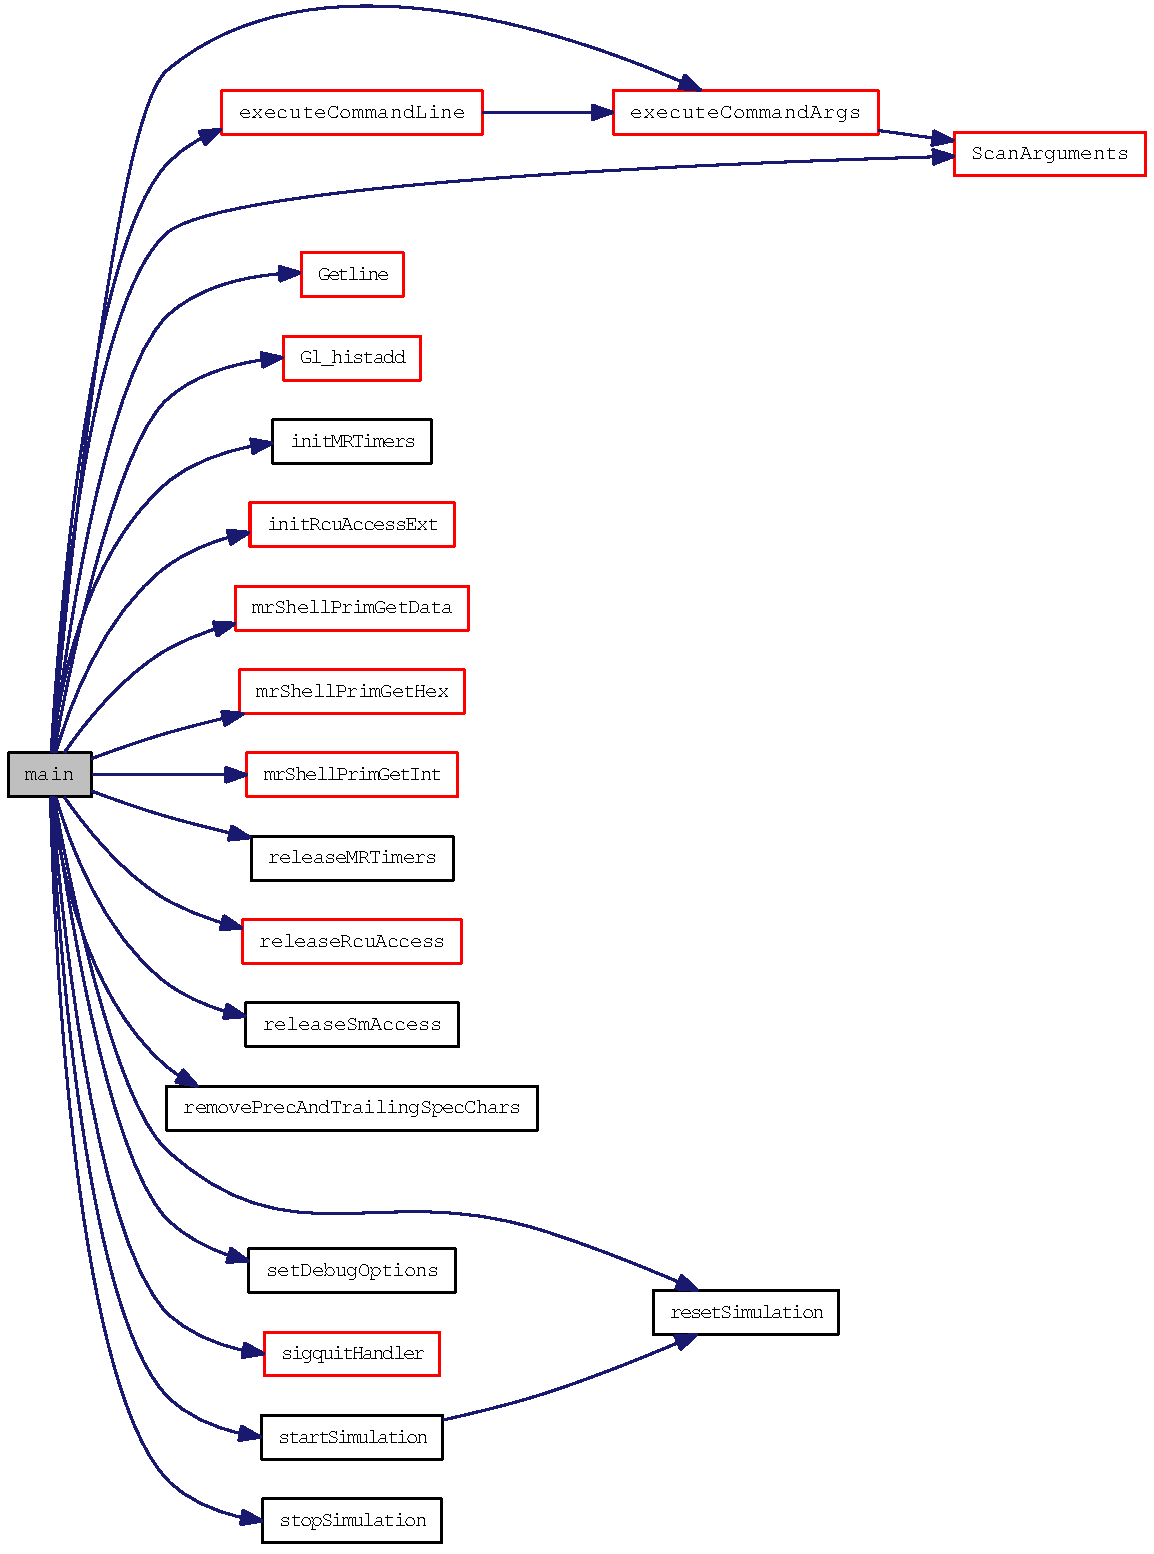
\includegraphics[width=295pt]{sendRCUcommand_8c_22ebaf74d5c7bacab58b44ae963c85d6_cgraph}
\end{center}
\end{figure}
\hypertarget{sendRCUcommand_8c_47cf995bed43c4e6bc563073f5b8f607}{
\index{sendRCUcommand.c@{send\-RCUcommand.c}!sigquitHandler@{sigquitHandler}}
\index{sigquitHandler@{sigquitHandler}!sendRCUcommand.c@{send\-RCUcommand.c}}
\subsubsection[sigquitHandler]{\setlength{\rightskip}{0pt plus 5cm}void sigquit\-Handler (int {\em param})}}
\label{sendRCUcommand_8c_47cf995bed43c4e6bc563073f5b8f607}




Definition at line 64 of file send\-RCUcommand.c.

References terminate\-Batch\-Processing().

Referenced by main().

Here is the call graph for this function:\begin{figure}[H]
\begin{center}
\leavevmode
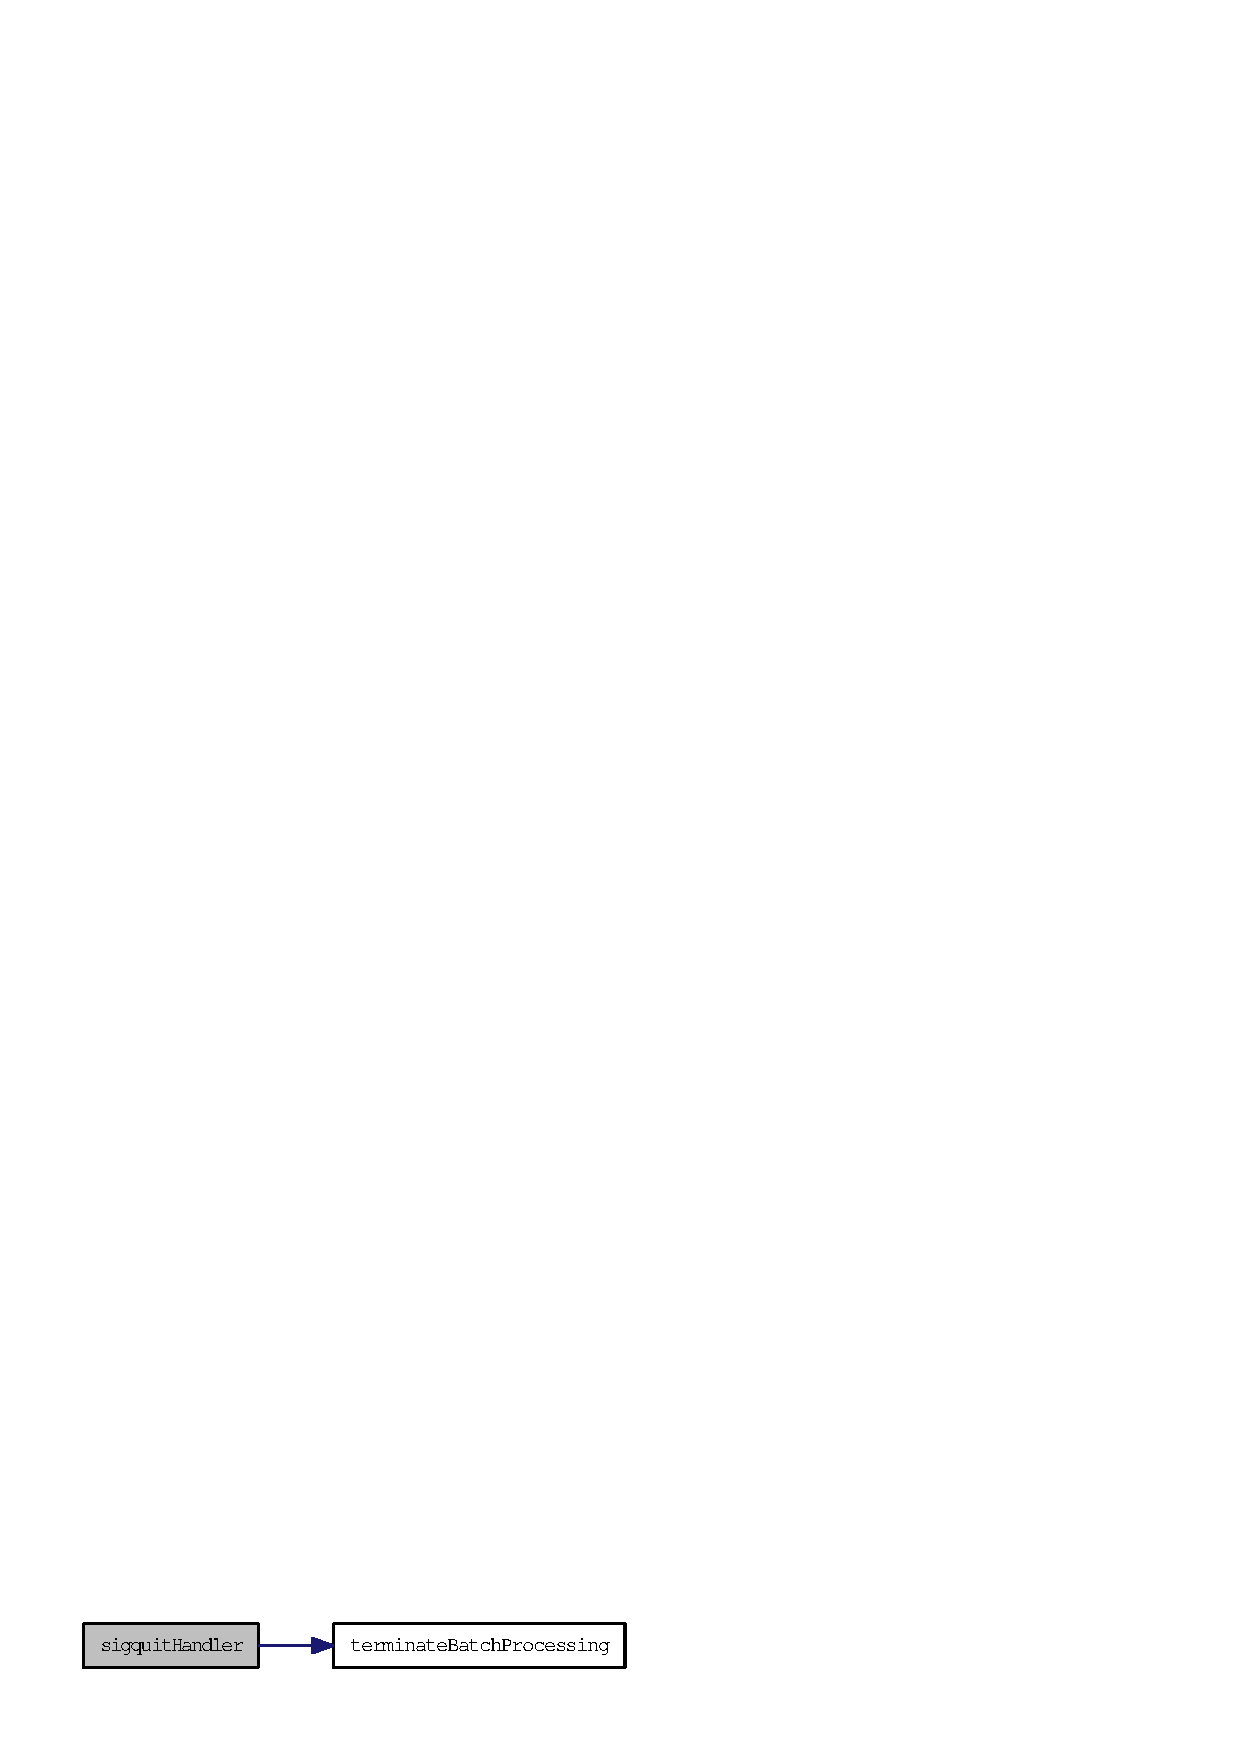
\includegraphics[width=152pt]{sendRCUcommand_8c_47cf995bed43c4e6bc563073f5b8f607_cgraph}
\end{center}
\end{figure}


\subsection{Variable Documentation}
\hypertarget{sendRCUcommand_8c_34fcfc606a53070425a87fce190ee38d}{
\index{sendRCUcommand.c@{send\-RCUcommand.c}!g_mrShellPrimDbg@{g\_\-mrShellPrimDbg}}
\index{g_mrShellPrimDbg@{g\_\-mrShellPrimDbg}!sendRCUcommand.c@{send\-RCUcommand.c}}
\subsubsection[g\_\-mrShellPrimDbg]{\setlength{\rightskip}{0pt plus 5cm}unsigned int \hyperlink{sendRCUcommand_8c_34fcfc606a53070425a87fce190ee38d}{g\_\-mr\-Shell\-Prim\-Dbg}}}
\label{sendRCUcommand_8c_34fcfc606a53070425a87fce190ee38d}




Definition at line 33 of file mrshellprim.c.

Referenced by call\-Command\-Handler(), Get\-Nof\-Required\-Args(), Is\-Separator(), mr\-Shell\-Prim\-Clear\-Debug\-Flag(), mr\-Shell\-Prim\-Set\-Debug\-Flag(), Read\-Argument(), Scan\-Arguments(), and Search\-Def().\hypertarget{sendRCUcommand_8c_641307208f220bf55de2578828522acd}{
\index{sendRCUcommand.c@{send\-RCUcommand.c}!mainArgs@{mainArgs}}
\index{mainArgs@{mainArgs}!sendRCUcommand.c@{send\-RCUcommand.c}}
\subsubsection[mainArgs]{\setlength{\rightskip}{0pt plus 5cm}\hyperlink{structArgDef__t}{TArg\-Def} \hyperlink{sendRCUcommand_8c_641307208f220bf55de2578828522acd}{main\-Args}\mbox{[}$\,$\mbox{]}}}
\label{sendRCUcommand_8c_641307208f220bf55de2578828522acd}


\textbf{Initial value:}

\begin{Code}\begin{verbatim} {
  {"--mrsdbg",NULL,{eHexArray, {(void*)&g_mrShellPrimDbg}},{(void*)1},0},
  {"--mrshelp",NULL,{eFctNoArg, {(void*)mrShellPrimPrintDbgFlags}},{(void*)1},ARGDEF_TERMINATE},
  {"-*","--*",{eFctInclusive, {(void*)mainOptions}},{(void*)&scanModeMainOptions},0},
  {NULL,NULL,{eBool, {NULL}},{NULL},ARGDEF_BREAK},
  {"","",{eUnknownType, {NULL}},{NULL},0},
}
\end{verbatim}\end{Code}


Definition at line 98 of file send\-RCUcommand.c.

Referenced by main().\hypertarget{sendRCUcommand_8c_3f74ad6fcd7825c54ac293c30f5c84dc}{
\index{sendRCUcommand.c@{send\-RCUcommand.c}!mainOptions@{mainOptions}}
\index{mainOptions@{mainOptions}!sendRCUcommand.c@{send\-RCUcommand.c}}
\subsubsection[mainOptions]{\setlength{\rightskip}{0pt plus 5cm}\hyperlink{structArgDef__t}{TArg\-Def} \hyperlink{sendRCUcommand_8c_3f74ad6fcd7825c54ac293c30f5c84dc}{main\-Options}\mbox{[}$\,$\mbox{]}}}
\label{sendRCUcommand_8c_3f74ad6fcd7825c54ac293c30f5c84dc}


\textbf{Initial value:}

\begin{Code}\begin{verbatim} {
  {"-d","--device=",{eConstString, {NULL}},{NULL},ARGDEF_UNTERM_LONG},
  {"-e","--encode",{eBool, {NULL}},{NULL},0},
  {"-a","--append",{eBool, {NULL}},{NULL},0},
  {"-v","--verbosity",{eInteger, {NULL}},{NULL},0},
  {NULL,"--debug",{eHex, {NULL}},{NULL},0},
  {NULL,"--mibsize",{eHex, {NULL}},{NULL},0},
  {"-mmgv","--memory-guard-verbosity",{eInteger, {NULL}},{NULL},0},
  {"-mmgf","--memory-guard-logfile",{eConstString, {NULL}},{NULL},0},
  {"-h","--help",{eFctNoArg, {(void*)printHelp}},{NULL},ARGDEF_TERMINATE},
  {"-i","--info",{eFctNoArg, {(void*)printInfo}},{NULL},ARGDEF_TERMINATE},
  {"","",{eUnknownType, {NULL}},{NULL},0},
}
\end{verbatim}\end{Code}


Definition at line 84 of file send\-RCUcommand.c.

Referenced by main().\hypertarget{sendRCUcommand_8c_bae7cc25bf2667a9438fbb8ca696ae75}{
\index{sendRCUcommand.c@{send\-RCUcommand.c}!scanModeMainOptions@{scanModeMainOptions}}
\index{scanModeMainOptions@{scanModeMainOptions}!sendRCUcommand.c@{send\-RCUcommand.c}}
\subsubsection[scanModeMainOptions]{\setlength{\rightskip}{0pt plus 5cm}\hyperlink{structFctMode__t}{TFct\-Mode} \hyperlink{sendRCUcommand_8c_bae7cc25bf2667a9438fbb8ca696ae75}{scan\-Mode\-Main\-Options} = \{SCANMODE\_\-FORCE\_\-TERMINATION$|$SCANMODE\_\-READ\_\-ONE\_\-CMD$|$SCANMODE\_\-PERSISTENT, NULL, NULL\}}}
\label{sendRCUcommand_8c_bae7cc25bf2667a9438fbb8ca696ae75}




Definition at line 75 of file send\-RCUcommand.c.\hypertarget{sendRCUcommand_8c_8481f9823ab837a716b4294324fd3def}{
\index{sendRCUcommand.c@{send\-RCUcommand.c}!scanModeNoError@{scanModeNoError}}
\index{scanModeNoError@{scanModeNoError}!sendRCUcommand.c@{send\-RCUcommand.c}}
\subsubsection[scanModeNoError]{\setlength{\rightskip}{0pt plus 5cm}\hyperlink{structFctMode__t}{TFct\-Mode} \hyperlink{sendRCUcommand_8c_8481f9823ab837a716b4294324fd3def}{scan\-Mode\-No\-Error} = \{SCANMODE\_\-SILENT$|$SCANMODE\_\-FORCE\_\-TERMINATION, NULL, NULL\}}}
\label{sendRCUcommand_8c_8481f9823ab837a716b4294324fd3def}




Definition at line 74 of file send\-RCUcommand.c.

Referenced by main().\hypertarget{sendRCUcommand_8c_260fedd682f84c2bf63d9fbcf7a85a84}{
\index{sendRCUcommand.c@{send\-RCUcommand.c}!scanModeShellArgs@{scanModeShellArgs}}
\index{scanModeShellArgs@{scanModeShellArgs}!sendRCUcommand.c@{send\-RCUcommand.c}}
\subsubsection[scanModeShellArgs]{\setlength{\rightskip}{0pt plus 5cm}\hyperlink{structFctMode__t}{TFct\-Mode} \hyperlink{sendRCUcommand_8c_260fedd682f84c2bf63d9fbcf7a85a84}{scan\-Mode\-Shell\-Args} = \{SCANMODE\_\-FORCE\_\-TERMINATION, \char`\"{} \char`\"{}, NULL\}}}
\label{sendRCUcommand_8c_260fedd682f84c2bf63d9fbcf7a85a84}




Definition at line 76 of file send\-RCUcommand.c.\hypertarget{sendRCUcommand_8c_c5dd9bf9adc293400bcf4c9746e1624d}{
\index{sendRCUcommand.c@{send\-RCUcommand.c}!shellArgs@{shellArgs}}
\index{shellArgs@{shellArgs}!sendRCUcommand.c@{send\-RCUcommand.c}}
\subsubsection[shellArgs]{\setlength{\rightskip}{0pt plus 5cm}\hyperlink{structArgDef__t}{TArg\-Def} \hyperlink{sendRCUcommand_8c_c5dd9bf9adc293400bcf4c9746e1624d}{shell\-Args}\mbox{[}$\,$\mbox{]}}}
\label{sendRCUcommand_8c_c5dd9bf9adc293400bcf4c9746e1624d}


\textbf{Initial value:}

\begin{Code}\begin{verbatim} {
  {"h","help",{eFctNoArg, {(void*)printHelp}},{NULL},ARGDEF_UNTERM_SHORT},
  {"info","i",{eFctNoArg, {(void*)printInfo}},{NULL},ARGDEF_UNTERM_SHORT},
  {"","",{eUnknownType, {NULL}},{NULL},0},
}
\end{verbatim}\end{Code}


Definition at line 78 of file send\-RCUcommand.c.